% !TEX TS-program = pdflatex
% !TEX encoding = UTF-8 Unicode
% !TEX ROOT = main.tex

\section*{Geschichtliches zu Universität, Fakultät und Fachschaft}

Im folgenden findet ihr eine kleine Auswahl an größeren und kleineren Umwälzungen, die der Universität und insbesondere der Physik in Heidelberg im Laufe der Jahrhunderte widerfahren sind. Für eine genaueren Einblick sei auf den Text zur Geschichte von Stadt und Universität in diesem Tagungsheft verwiesen.

\begin{wrapfigure}[]{r}{3cm}
\vspace{-13pt}
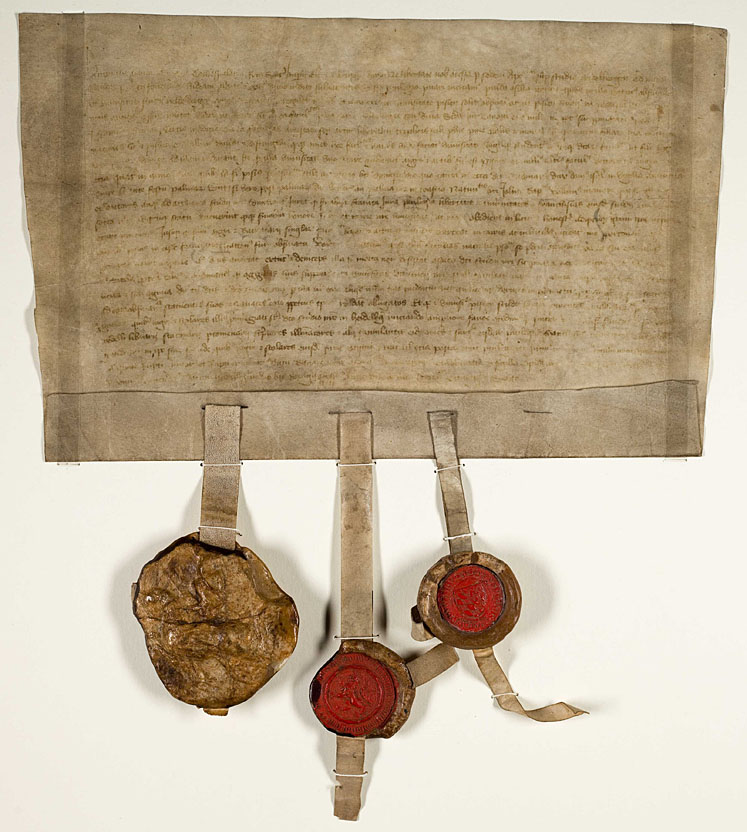
\includegraphics[width=3cm]{urkunde.jpg}

\small{Gründungsurkunde}
\end{wrapfigure}

\textbf{1386} Der pfälzische Kurfürst Ruprecht I. gründet auf Weisung des Papstes in Heidelberg die dritte Universität des Heiligen Römischen Reichs deutscher Nation\\
\textbf{1387}  Erste Physik-Vorlesung (im aristotelesschen Sinne)\\
\textbf{1693} Die Truppen von Ludwig XIV. zerstören die Stadt, wie man bis heute am Schloss erkennen kann\\
\textbf{1752} Einrichtung eines Lehrstuhls für experimentelle und mathematische Physik\\
\textbf{1806} Unter dem badischen Großherzog Karl-Friedrich wird die Uni reorganisiert, seit dem nennt sie sich Ruprecht-Karls-Universität (Ruperto Carola)

\begin{wrapfigure}{l}{3cm}
\vspace{-13pt}
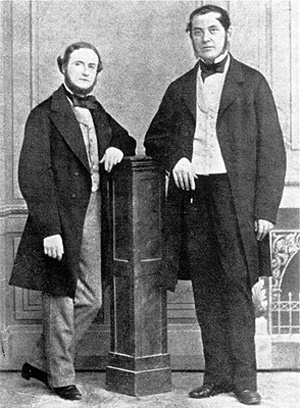
\includegraphics[width=3cm, height=3.95cm]{kirchhoff.jpg}
\small{Bunsen \& Kirchhoff}
\vspace{-13pt}
\end{wrapfigure}

\textbf{1859} Gustav Kirchhoff und Robert Bunsen entdecken die Spektralanalyse\\
\textbf{1890} Abtrennung der Naturwissenschaftlich-Mathematischen Fakultät von der Philosophischen Fakultät\\
\textbf{1900} Erstmals dürfen im Land Baden und somit auch in Heidelberg Frauen studieren\\
\textbf{1913} Das Physikalische Institut am Philosophenweg 12 wird eröffnet\\
\textbf{1933} Ab der Machtübernahme kommt es zur Entlassung von etwa einem Drittel des gesamten Lehrkörpers. Studierende kritischer Gesinnung werden zwangsexmatrikuliert. 

\begin{wrapfigure}{r}{3.5cm}
\vspace{-13pt}
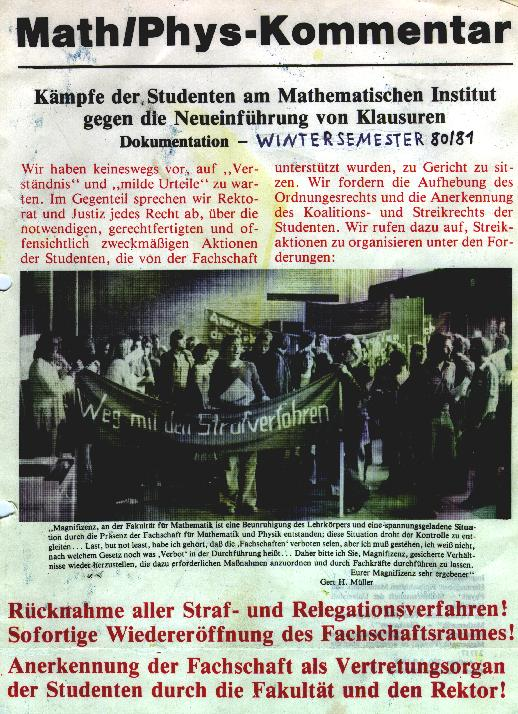
\includegraphics[width=3.5cm]{prozesse.jpg}
\small{Klausuren sorgten für Unruhen}
\vspace{5pt}
\end{wrapfigure}

\textbf{1970} Einrichtung einer eigenständigen Fakultät für Physik und Astronomie\\
\textbf{1977} Die verfasste Studierendenschaft in Baden-Württemberg wird abgeschafft\\
\textbf{1977} An der Mathematik-Fakultät sollen in Erstsemestervorlesungen Klausuren eingeführt werden.
Die Fachschaft MathPhys organisiert verschiedenste Protestaktionen gegen diese Pläne. In Folge dessen kommt es zu Strafprozessen und Verurteilungen gegen Mitglieder der Fachschaft. Das Rektorat veranlasst die Schließung des Fachschaftsraums.\\
\textbf{1980} Die Fachschaft erstreitet einen Raum im Theoretikum\\
\textbf{1994} Winter-ZaPF in HD (\#34)\\
\textbf{1996} Erstes MathPhysRom-Fest der Fachschaften Physik, Mathematik und Romanistik

\begin{wrapfigure}{l}{3cm}
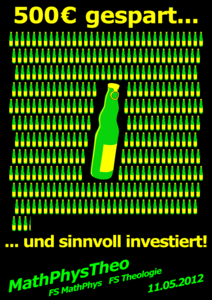
\includegraphics[width=3cm]{500.png}
\small{Festmotto 2012}
\end{wrapfigure}
\textbf{2002} Winter-Zapf in HD (\#47)\\
\textbf{2002} Eröffnung des Kirchhoff-Instituts für Physik, Umzug der Experimentalphysik ins Neuenheimer-Feld\\
\textbf{2007} Die Uni ist erstmalig in ihrer sechshundertjährigen Geschichte exzellent\\
\textbf{2011} Aus MathPhysRom wird MathPhysTheo, die Theologie löst die Romanistik ab\\
\textbf{2012} Die 2007 eingeführten allgemeinen Studiengebühren werden abgeschafft\\
\textbf{2013} Die Verfasste Studierendenschaft wird wieder im LHG eingeführt, Fachschaftswahlen sind wieder legal\\
\textbf{2016} Umzug des Fachschaftsraums vom Theoretikum in das Mathematikon, eins von vielen Gebäuden, welches die Uni der Klaus-Tschira-Stiftung verdankt\\
\textbf{2017} Studiengebühren für Nicht-EU-Ausländer und Zweitstudierende werden eingeführt\\
\textbf{2018} Sommer-ZaPF in HD (\#78)
\subsection*{NS-Zeit und deutsche Physik}
\begin{wrapfigure}{r}[0cm]{4cm}
\vspace{-13pt}
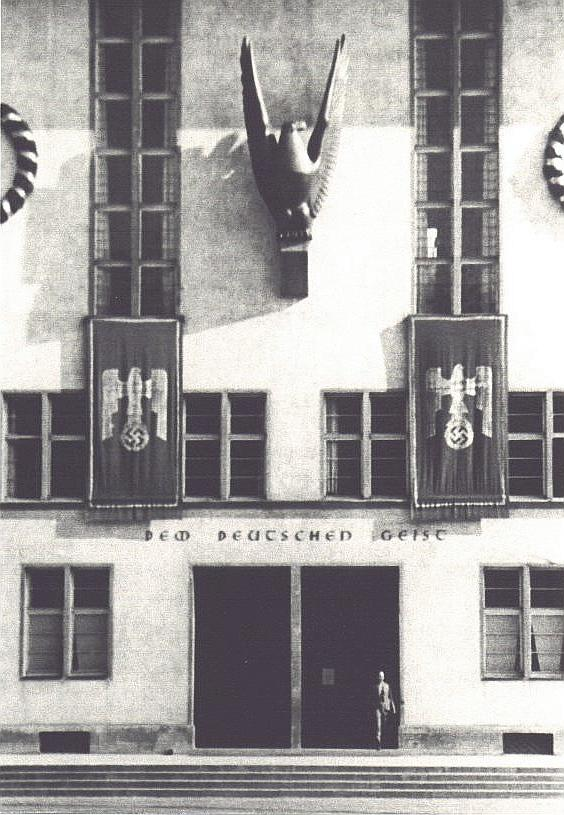
\includegraphics[width=4cm]{deutschergeist.jpg}
\small{1936: Reichsadler über dem Eingang zur neuen Universität und der Inschrift: \textit{dem deutschen Geist}}
\vspace{-15pt}
\end{wrapfigure}

Schnell geriet unsere Uni als \textit{braune Universität} in Verruf. Nationalsozialistisch eingestellte Studenten, ihre Burschenschaften sowie Teile der Professorenschaft hatten den Boden für den Aufstieg der Nationalsozialisten bereitet, so dass man bei der Machtübernahme schon größtenteils auf Linie war.\\
Die Physik nahm bei der Verflechtung von Wissenschaft und rassistischer Ideologie eine Vorreiterrolle ein und ließ früh jegliche Ansprüche an Neutralität und wissenschaftlichen Ethos vermissen.

Mit der Machterübernahme der Faschisten im Jahre 1933 wurden mehr als 25\% der in akademischen Positionen tätigen Physiker*innen in Deutschland aus rassistischen oder politischen Gründen entlassen, in Heidelberg war dies in diesem Ausmaß nicht mehr nötig, denn hier lehrte und forschte man seit Längerem nach den Grundsätzen einer \textit{deutschen und arischen Physik}.

Als einer ihrer Begründer gilt Philipp Lenard, Nobelpreis 1905 und Direktor des Physikalischen Instituts seit 1907. 
Seine Zeiten als einfallsreicher Experimentator hatte er schon hinter sich, nun widmete er sich unter Anderem der Verteidigung eines Ätherkonzepts, welches durch die vorschanreitenden Erkenntnisse der Relativitätstheorie und Quantenmechanik obsolet wurde. Die moderne Physik lehnte er als falsch und unintuitiv ab und entwickelte so im Laufe der Jahre eine persönliche Feindschaft zu Albert Einstein, wobei er zunehmends antisemitisch argumentierte und die \textit{jüdischen Einflüsse in der Wissenschaft} beklagte. Bereits 1924 sprach er sich in der Großdeutschen Zeitung öffentlich für Hitler aus und missbrauchte Zeit seiner Vorlesungen für Lobreden auf Hitler.

Als Institutsdirektor nahm Lenard erheblichen Einfluss auf Forschungsschwerpunkte, Berufungsverfahren und die Physik in Deutschland allgemein, auch nach seiner Emeritierung 1931, stets im Sinne einer \textit{arischen Naturforschung}. Assistenten wurden angewiesen am laufenden Band Artikel gegen Relativitätstheorie und Quantenmechanik zu veröffentlichen. Die physikalischen Gewissheiten sprachen zu dem Zeitpunkt bereits eine ganz andere Sprache, und ohne die moderne \textit{jüdische} Physik wäre auch das spätere Uranprojekt der Nazis nicht möglich gewesen. 

Ab 1933 widmete man Bereiche der Forschung explizit militärischen Zielen, in der neu gegründeten physikalisch-technischen Abteilung war wehrwissentschaftlicher Untericht Teil der Lehre, man forschte zu Funktechnik, Bildübertragung und im Laufe des Krieges zu Tarntechniken. Die SS soll zeitweise auf dem Dachboden des Gebäudes exerziert haben.
Um den \textit{deutschen Vorzeigewissenschaftler} Lenard wurde ein Personenkult inszeniert, das Institut wurde 1935 sogar nach ihm benannt, Studierende organisierten Fackelmärsche vor seiner Haustür zu seinem Geburtstag. 

Gegen Ende der NS-Diktatur spielte die deutsche Physik praktisch keine Rolle mehr und heute wird sie oft aufgrund ihrer offensichtlichen Absurdität belächelt.\\ Allerdings soll dieses dunkle Kapitel in der Geschichte der Universität noch lange als Warnung für Generationen von zukünftigen Wissenschaftler*innen dienen, sich nicht für menschenverachtende Ziele vereinnahmen zu lassen und den moralischen Kredit der Wissenschaft zu verspielen.

%BILDQUELLEN
%http://www.ub.uni-heidelberg.de/bilder/ausstellung/625unihd/virtuelleausstellung/exponate/sektion1/01_05.jpg
%https://upload.wikimedia.org/wikipedia/commons/0/0e/Bunsen-Kirchhoff.jpg
%https://mathphys.fsk.uni-heidelberg.de/w/wp-content/uploads/mathphyskommentartitel.jpg
%http://www.tphys.uni-heidelberg.de/Ausstellung/show.cgi?P=deD22155
